\chapter{芳香性与亲电芳香取代}\label{ch:b2:aromatic-substitution}

溴水与烯烃振荡后数秒内即褪色，
而与苯则完全不褪色。然而苯与溴在
加入少量溴化铁（III）后即可反应——生成的溴苯
仍保留其六元芳香环：只是一个氢原子被取代，
并未发生加成。芳环以取代而非加成的方式反应，因为加成
将丢失在\cref{ch:b2:huckel}中计算得到的稳定化能。同一机理
可使苯环发生硝化、磺化、烷基化和酰基化，
且环上已有的基团会以惊人的规律决定
下一个基团进入的位置。

\begin{recall}
\Cref{ch:b2:huckel}：苯的芳香性与\omterm{def:b2:huckel:delocalisation}{离域能}。本科一年级
分册：烯烃的亲电加成、诱导效应与共轭效应、给电子基团和
吸电子基团、碳正离子及其重排、哈蒙德假设、路易斯酸、
能量曲线。
\end{recall}

\begin{omfigure}
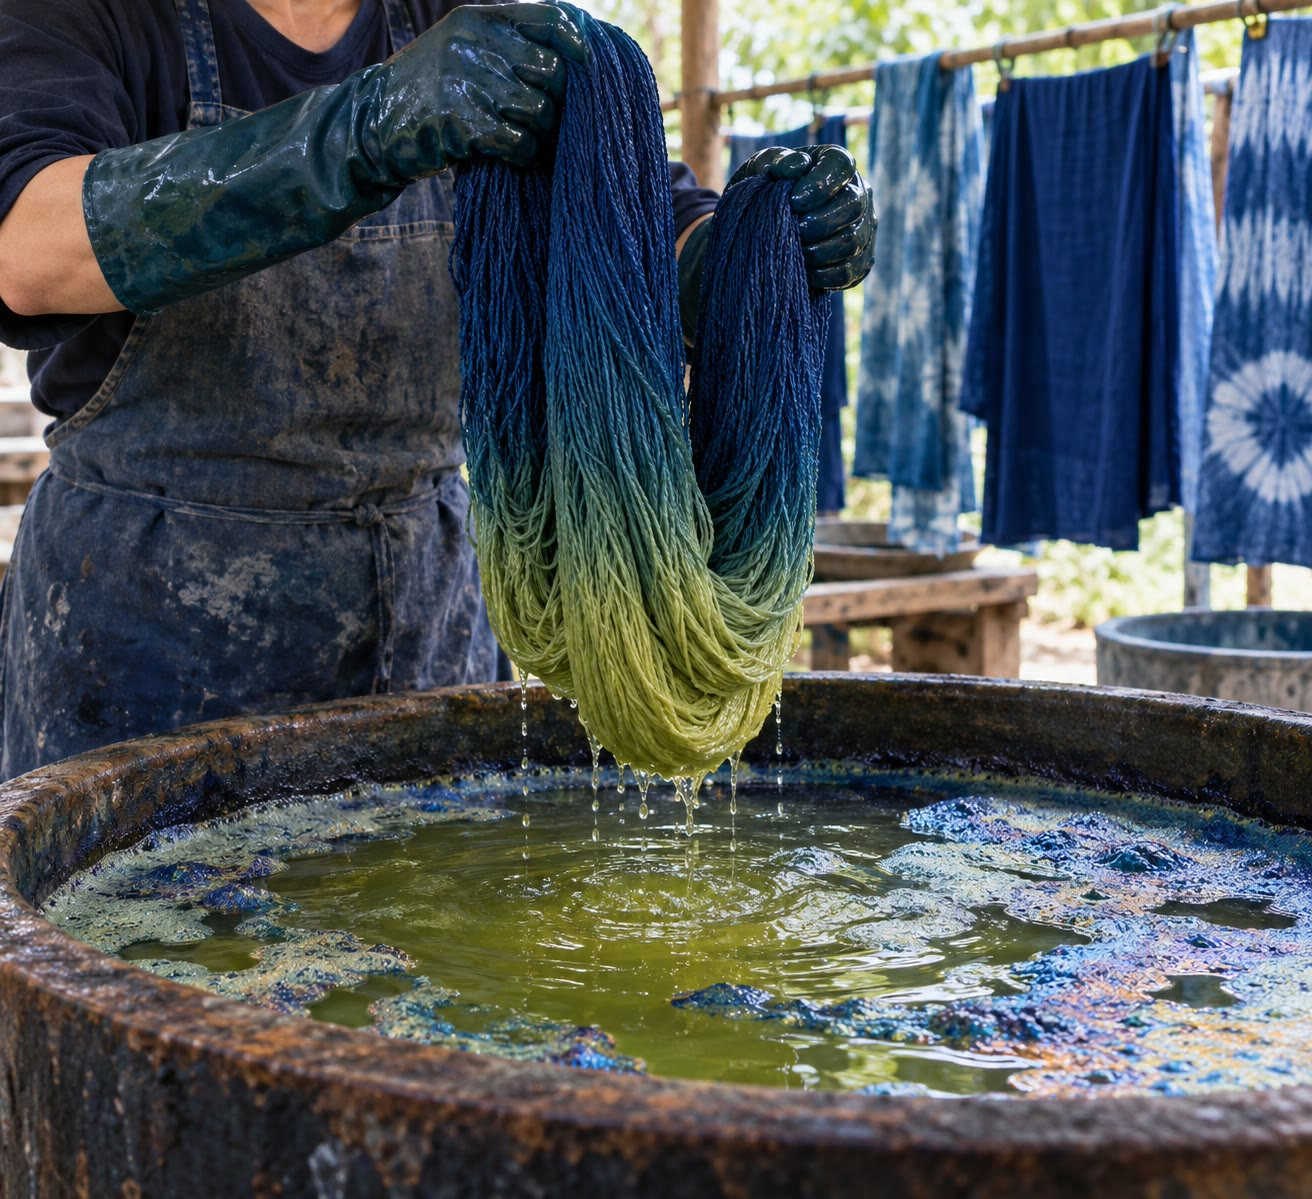
\includegraphics[width=0.55\linewidth]{images/book3/ai/b2-22-indigo-vat-2.jpg}

{\small 在靛蓝染缸中染纱线（示意图）。纱线离开染缸时呈黄绿色，浸透了
染料的可溶还原态，在空气中显蓝色，氧使其重新变为
不溶的靛蓝。靛蓝与多数染料一样，以芳环为骨架；
十九世纪的染料工业由本章所述取代反应发展而来，
将其应用于来自煤焦油的苯。}
\end{omfigure}

\section{取代而非加成}

\begin{definition}[芳烃]\label{def:b2:aromatic-substitution:arene}
\emph{芳烃}\index{芳烃}是指至少含有一个芳环的烃，例如
苯、甲苯（甲基苯）或萘；芳基（\ce{Ar}）即去掉
一个氢原子的芳烃。
\end{definition}

\begin{proposition}[为何苯不发生加成]\label{prop:b2:aromatic-substitution:no-addition}
苯若发生加成，芳环将变为非\omterm{def:b2:huckel:aromatic}{芳香性的}环己二烯，并
失去其中大部分\qty{150}{kJ/mol}的芳香稳定化能；取代则保留了它。
\end{proposition}

\begin{proof}[论证]
在\cref{ch:b2:huckel}中，苯加氢生成环己-1,3-二烯
被测得为吸热过程（\qty{+22}{kJ/mol}，由\qty{-206.0}{}与\qty{-227.7}{kJ/mol}推得），而普通
双键加成放出\qty{119}{kJ/mol}：第一步加成是代价高昂的一步。
第一步亲电步骤之后，生成的阳离子既可加合亲核试剂，
形成非芳香的二烯，也可失去质子而恢复芳环。第二条
途径有利得多。
% ledger: dfh:C6H6_g, dfh:C6H8_g, dfh:C6H10_g, dfh:C6H12_g
\end{proof}

\section{反应机理}

\begin{definition}[亲电芳香取代]\label{def:b2:aromatic-substitution:seAr}
\emph{亲电芳香取代}\index{亲电芳香取代}是指
用亲电试剂 \ce{E+} 取代芳环上的一个氢原子。亲电试剂先
与环上某一个碳原子成键，生成一个阳离子，其中该碳为四面体构型，
正电荷分散在其余五个碳原子上，称为\emph{惠兰德中间体}\index{惠兰德中间体}
（芳正离子）。随后碱从该四面体碳原子上夺去质子。
\end{definition}

\begin{proposition}[两步反应]\label{prop:b2:aromatic-substitution:mechanism}
第一步破坏芳香性，是慢的一步；失去质子
恢复\omterm{def:b2:huckel:aromatic}{芳香性的}那一步则是快的。
\end{proposition}

\begin{proof}[论证]
\omterm{def:b2:aromatic-substitution:seAr}{惠兰德中间体}是一种碳正离子，由三个碳原子上的离域作用而稳定，
但不具芳香性，能量远高于反应物；由哈蒙德假设，通向它的
过渡态在结构和能量上都与其相近。第二步
生成芳香性产物，能垒很低。
\end{proof}

\begin{omfigure}
\begin{tikzpicture}
\begin{axis}[width=0.55\linewidth, height=5.4cm, xmin=-0.2, xmax=4.2, ymin=-5.5, ymax=11.5,
  axis x line=bottom, axis y line=left, xtick=\empty, ytick=\empty,
  xlabel={反应坐标}, ylabel={能量}, label style={font=\small}, clip=false]
\addplot[omDef, thick] table[x=x, y=sub] {figdata/out/bachelor-2-aromatic-profile.dat};
\addplot[omThm, thick, dashed, restrict x to domain=2:4] table[x=x, y=add] {figdata/out/bachelor-2-aromatic-profile.dat};
\node[font=\scriptsize, anchor=north west] at (axis cs:0.0,-0.6) {反应物 \ce{ArH + E+}};
\node[font=\scriptsize, anchor=north] at (axis cs:2,5.7) {惠兰德中间体};
\node[font=\scriptsize, anchor=west, omDef] at (axis cs:4.05,-4.0) {生成物 \ce{ArE + H+}};
\node[font=\scriptsize, anchor=west, omThm] at (axis cs:4.05,2.0) {加成产物};
\node[font=\scriptsize, anchor=south] at (axis cs:1,10.1) {慢};
\end{axis}
\end{tikzpicture}

{\small \omterm{def:b2:aromatic-substitution:seAr}{亲电芳香取代}的能量曲线，示意图（模型）。
第一步生成\omterm{def:b2:aromatic-substitution:seAr}{惠兰德中间体}，能垒最高。失去
一个质子（实线）使芳环复原；加合亲核试剂（虚线）则
将得到一个高于反应物能量的产物。}
\end{omfigure}

\begin{omfigure}
\setchemfig{atom sep=2em}
\schemestart
\chemfig{HO-\chemabove{N}{\scriptstyle +}(=[1]O)-[7]\chemabove{O}{\scriptstyle -}} \+ \chemfig{H_2SO_4}
\arrow{<=>}
\chemfig{O=N^{+}=O} \+ \chemfig{HSO_4^{-}} \+ \chemfig{H_2O}
\schemestop

\medskip
\begin{tikzpicture}[font=\small, >={Stealth}]
\tikzset{pics/whel/.style n args={4}{code={
    \foreach \k in {0,...,5} \draw[thick] ({90+60*\k}:0.7) -- ({150+60*\k}:0.7);
    \foreach \k in {#1} \draw[thick] ($({90+60*\k}:0.56)!0.18!({150+60*\k}:0.56)$) -- ($({90+60*\k}:0.56)!0.82!({150+60*\k}:0.56)$);
    \ifnum#2>-1 \node[font=\scriptsize] at ({90+60*#2}:0.36) {$+$};\fi
    \draw[thick] (270:0.7) -- ++(-125:0.42) node[anchor=north east, inner sep=1pt, font=\scriptsize] {H};
    \draw[thick] (270:0.7) -- ++(-55:0.42) node[anchor=north west, inner sep=1pt, font=\scriptsize] {#4};
    \if\relax\detokenize{#3}\relax\else
      \draw[thick] (90:0.7) -- (90:1.1) node[anchor=south, inner sep=1pt, font=\scriptsize] {#3};\fi
  }}}
  \foreach \k in {0,...,5} \draw[thick] ({90+60*\k}:0.7) -- ({150+60*\k}:0.7);
  \foreach \k in {0,2,4} \draw[thick] ($({90+60*\k}:0.56)!0.18!({150+60*\k}:0.56)$) -- ($({90+60*\k}:0.56)!0.82!({150+60*\k}:0.56)$);
  \node at (1.3,0) {$+$};
  \node at (2.0,0) {\ce{NO2+}};
  \draw[->, thick] (2.6,0) -- (3.8,0) node[midway, above, font=\scriptsize] {慢};
  \pic at (4.7,0.1) {whel={1,4}{0}{}{\ce{NO2}}};
  \draw[->, thick] (5.6,0) -- (6.8,0) node[midway, above, font=\scriptsize] {快} node[midway, below, font=\scriptsize] {$-$\ce{H+}};
  \begin{scope}[xshift=7.7cm]
    \foreach \k in {0,...,5} \draw[thick] ({90+60*\k}:0.7) -- ({150+60*\k}:0.7);
    \foreach \k in {0,2,4} \draw[thick] ($({90+60*\k}:0.56)!0.18!({150+60*\k}:0.56)$) -- ($({90+60*\k}:0.56)!0.82!({150+60*\k}:0.56)$);
    \draw[thick] (270:0.7) -- (270:1.1) node[anchor=north, font=\scriptsize] {\ce{NO2}};
  \end{scope}
\end{tikzpicture}
\par\vspace{6pt}

{\small 苯的硝化。硫酸使硝酸质子化，后者失去水，
生成硝酰正离子 \ce{NO2+}，是亲电试剂。它与一个碳原子成键（慢），生成
\omterm{def:b2:aromatic-substitution:seAr}{惠兰德中间体}，其正电荷分布于整个环上；失去一个质子
（快）得到硝基苯。}
\end{omfigure}

\section{反应}

\paragraph{卤化。} 单独的溴或氯作为亲电试剂太弱；路易斯酸
（\ce{FeBr3}、\ce{AlCl3}）通过与卤素的一个原子结合而使其极化，
外侧的溴原子进攻苯环。

\paragraph{硝化。} 浓硝酸与浓硫酸的混合物（见上文）生成
硝酰正离子。

\paragraph{磺化。} 发烟硫酸（\ce{SO3} 溶于 \ce{H2SO4}）生成苯磺酸。
反应可逆：将磺酸在稀的酸性水溶液中加热，可使
\ce{SO3H} 基团重新脱去，因此它是一种有用的临时封闭基团。

\begin{definition}[傅–克反应]\label{def:b2:aromatic-substitution:friedel-crafts}
称\emph{傅–克烷基化}\index{傅–克烷基化}为在路易斯酸
（\ce{AlCl3}）作用下，由卤代烷将烷基引入芳环的反应。
\emph{傅–克酰基化}\index{傅–克酰基化}则是将酰基
\ce{RCO} 由酰氯与 \ce{AlCl3} 作用引入，经\emph{酰基正离子}\index{酰基正离子}
\ce{R-C#O+}，生成芳基酮。
\end{definition}

\begin{proposition}[傅–克反应的局限性]\label{prop:b2:aromatic-substitution:friedel-crafts-limits}
\omterm{def:b2:aromatic-substitution:friedel-crafts}{傅–克烷基化}的缺点在于碳正离子的重排，以及
多烷基化的问题；酰基化在一次取代后即停止，不发生重排，并且需要
至少一当量的 \ce{AlCl3}。两者均不适用于带有强
\omterm{def:b2:aromatic-substitution:directing}{钝化基团}的芳环。
\end{proposition}

\begin{proof}[论证]
烷基化的亲电试剂是碳正离子（或行为类似碳正离子的配合物），
它通过氢负离子或烷基的迁移，重排为更稳定的碳正离子：1-氯丙烷主要
得到异丙苯。烷基使芳环活化（见下节），因此产物
比苯更易反应，并再次被烷基化。\omterm{def:b2:aromatic-substitution:friedel-crafts}{酰基正离子}
通过共振（\ce{R-C+=O} $\leftrightarrow$ \ce{R-C#O+}）而稳定，不发生重排；酰基使
芳环\omterm{def:b2:corrosion:passivation}{钝化}，因此产物不再反应；生成的酮通过其氧原子与
\ce{AlCl3} 结合，将催化剂移出反应：一当量被
消耗。强\omterm{def:b2:corrosion:passivation}{钝化}的环作为亲核试剂过弱，难以与这些弱亲电试剂反应。
\end{proof}

\section{取代基效应}

\begin{definition}[定位基]\label{def:b2:aromatic-substitution:directing}
苯环上的取代基使环比苯更易反应时，称为\emph{活化基团}\index{活化基团}；
使环反应更慢时，称为\emph{钝化基团}\index{钝化基团}。
若新基团主要进入其邻位和对位，则称为\emph{邻/对位定位基}\index{邻/对位定位基}，
若主要进入间位，则称为\emph{间位
定位基}\index{间位定位基}。
\end{definition}

\begin{proposition}[给电子基团与吸电子基团]\label{prop:b2:aromatic-substitution:directing}
通过共轭效应向环供给电子的基团（\ce{-OH}、\ce{-OCH3}、\ce{-NH2}、
\ce{-NHCOCH3}）或通过诱导效应与\omterm{def:b2:fragment-orbitals:hyperconjugation}{超共轭}（烷基）使环活化，并使新基团进入
邻/对位。通过共轭效应吸电子的基团（\ce{-NO2}、\ce{-CN}、\ce{-COR}、
\ce{-COOH}、\ce{-SO3H}）使环\omterm{def:b2:corrosion:passivation}{钝化}，并使新基团进入间位。
\end{proposition}

\begin{proof}
比较\omterm{def:b2:aromatic-substitution:seAr}{惠兰德中间体}。进攻发生在取代基 G 的邻位或对位时，三个
共振结构之一使正电荷位于连有 G 的碳原子上；对间位进攻时，
三个结构均不如此。给电子基 G（O 或 N 上的孤电子对）使其所连的碳上的正电荷稳定，
并增加第四个共振结构，其中每个原子都满足八隅体：邻位和对位的
中间体能量降低，根据哈蒙德假设，通向它们的过渡态也随之降低。
吸电子基 G 使其所连碳上的正电荷不稳定：邻位和对位
中间体能量升高，而避开该结构的间位进攻所受不利最小，
但仍慢于苯。
\end{proof}

\begin{omfigure}
\begin{tikzpicture}[font=\small]
\tikzset{pics/whel/.style n args={4}{code={
    \foreach \k in {0,...,5} \draw[thick] ({90+60*\k}:0.7) -- ({150+60*\k}:0.7);
    \foreach \k in {#1} \draw[thick] ($({90+60*\k}:0.56)!0.18!({150+60*\k}:0.56)$) -- ($({90+60*\k}:0.56)!0.82!({150+60*\k}:0.56)$);
    \ifnum#2>-1 \node[font=\scriptsize] at ({90+60*#2}:0.36) {$+$};\fi
    \draw[thick] (270:0.7) -- ++(-125:0.42) node[anchor=north east, inner sep=1pt, font=\scriptsize] {H};
    \draw[thick] (270:0.7) -- ++(-55:0.42) node[anchor=north west, inner sep=1pt, font=\scriptsize] {#4};
    \if\relax\detokenize{#3}\relax\else
      \draw[thick] (90:0.7) -- (90:1.1) node[anchor=south, inner sep=1pt, font=\scriptsize] {#3};\fi
  }}}
  \node[anchor=east] at (-1.0,0) {甲氧基，对位进攻：};
  \pic at (0,0) {whel={1,4}{0}{\ce{OCH3}}{E}};
  \node at (1.25,0.1) {$\leftrightarrow$};
  \begin{scope}[xshift=2.5cm]
    \foreach \k in {0,...,5} \draw[thick] ({90+60*\k}:0.7) -- ({150+60*\k}:0.7);
    \foreach \k in {1,4} \draw[thick] ($({90+60*\k}:0.56)!0.18!({150+60*\k}:0.56)$) -- ($({90+60*\k}:0.56)!0.82!({150+60*\k}:0.56)$);
    \draw[thick] (-0.06,0.7) -- (-0.06,1.1); \draw[thick] (0.06,0.7) -- (0.06,1.1);
    \node[anchor=south, inner sep=1pt, font=\scriptsize] at (0,1.1) {$\overset{+}{\mathrm O}\mathrm{CH_3}$};
    \draw[thick] (270:0.7) -- ++(-125:0.42) node[anchor=north east, inner sep=1pt, font=\scriptsize] {H};
    \draw[thick] (270:0.7) -- ++(-55:0.42) node[anchor=north west, inner sep=1pt, font=\scriptsize] {E};
  \end{scope}
  \node[anchor=west, font=\scriptsize] at (3.4,0) {额外共振结构，各原子满足八隅体};
  \begin{scope}[yshift=-3.5cm]
    \node[anchor=east] at (-1.0,0) {硝基，对位进攻：};
    \pic at (0,0) {whel={1,4}{0}{\ce{NO2}}{E}};
    \node[anchor=west, font=\scriptsize] at (1.0,0) {正电荷位于连有吸电子基的碳上};
  \end{scope}
\end{tikzpicture}

{\small 对取代基进行对位进攻时的\omterm{def:b2:aromatic-substitution:seAr}{惠兰德中间体}。甲氧基时，氧原子的一对孤电子对
分担正电荷（多一个共振结构，各原子均满足八隅体）：
中间体得到稳定，该取代基使环活化，并为\omterm{def:b2:aromatic-substitution:directing}{邻/对位定位基}。对于硝基，
一个共振结构使正电荷位于连有吸电子基的
碳上：中间体不稳定，进攻转向间位。}
\end{omfigure}

\begin{proposition}[卤素]\label{prop:b2:aromatic-substitution:halogens}
卤素取代基使环\omterm{def:b2:corrosion:passivation}{钝化}，却为\omterm{def:b2:aromatic-substitution:directing}{邻/对位定位基}。
\end{proposition}

\begin{proof}[论证]
其诱导吸电子作用（源于电负性）降低了整个环的电子密度，
使每次进攻都变慢：\omterm{def:b2:corrosion:passivation}{钝化}作用。但卤素的一对孤电子对仍可
分担邻位与对位\omterm{def:b2:aromatic-substitution:seAr}{惠兰德中间体}的正电荷，这是间位中间体所不能的：
在这些变慢的进攻中，邻位与对位仍是最不慢的。
\end{proof}

\section{多取代苯}

\begin{method}[预测取代位置]\label{met:b2:aromatic-substitution:predict-position}
\begin{enumerate}
  \item 对每个取代基，标出其所偏好的位置（邻/对位或间位）。
  \item 若二者一致，则该位置胜出；若二者不一致，则由较强的活化基决定
        （\ce{-NH2}、\ce{-OH} $>$ \ce{-OCH3} $>$ \ce{-NHCOCH3} $>$ 烷基 $>$ 卤素）。
  \item 避开处于 1,3-位关系的两个取代基之间的位置（受阻），并且
        当基团体积较大时，预期对位优于邻位。
\end{enumerate}
\end{method}

\begin{method}[芳香化合物的合成规划]\label{met:b2:aromatic-substitution:plan-aromatic}
\begin{enumerate}
  \item 选择各步骤的先后次序，使已存在的每个基团都能在所需位置上引导下一步反应：
        要制得 3-溴硝基苯，应先硝化（\omterm{def:b2:aromatic-substitution:directing}{间位定位基}），再溴化；
        要制得 4-溴硝基苯，则应先溴化。
  \item 使用可转化基团：酰基（间位）可还原为烷基（邻/对位）；
        硝基（间位）还原为胺（邻/对位）；烷基氧化为
        \ce{-COOH}（间位）。
  \item 用 \ce{-SO3H} 占据某一位置，最后再将其除去。
  \item 缓和强活化基：胺在硝化或卤化之前先被酰化（\ce{-NHCOCH3}），
        随后再将其恢复。
\end{enumerate}
\end{method}

\begin{history}[傅里德尔与克拉夫茨]
\begin{minipage}[t]{0.18\linewidth}
\vspace{0pt}
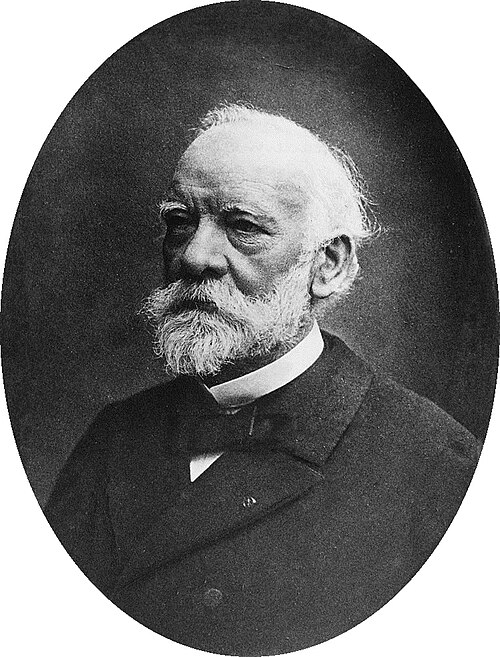
\includegraphics[width=\linewidth]{images/book3/friedel.jpg}
\end{minipage}\hspace{0.02\linewidth}%
\begin{minipage}[t]{0.18\linewidth}
\vspace{0pt}
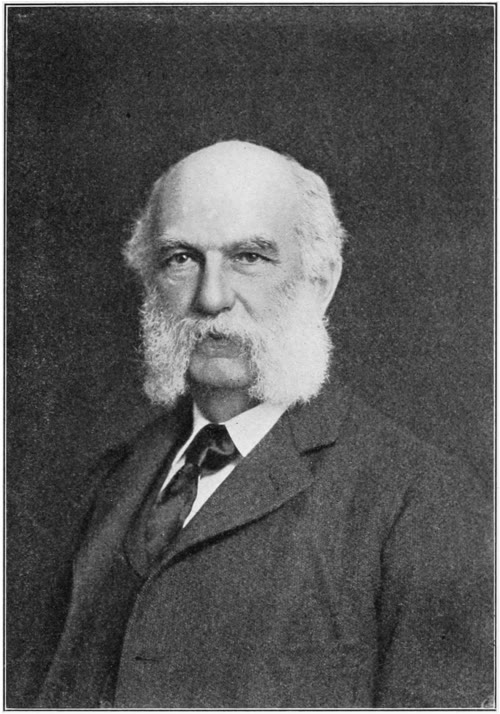
\includegraphics[width=\linewidth]{images/book3/crafts.jpg}
\end{minipage}\hfill
\begin{minipage}[t]{0.58\linewidth}
\vspace{0pt}
1877 年，查尔斯·傅里德尔与詹姆斯·梅森·克拉夫茨在巴黎合作，发现
氯化铝可使卤代烷和酰氯与苯发生反应。二人的
反应成为将碳基团连接到芳环上的标准方法，而他们发现的路易斯
酸催化作用的影响远超于此。（肖像：傅里德尔，1890 年代；克拉夫茨，取自
《大众科学月刊》，1900 年；公有领域，维基共享资源。）
\end{minipage}
\end{history}

\begin{safety}{\ghs[5mm]{GHS02}\,\ghs[5mm]{GHS05}\,\ghs[5mm]{GHS06}\,\ghs[5mm]{GHS08}}
苯是致癌物，凡有可能均以甲苯或其他\omterm{def:b2:aromatic-substitution:arene}{芳烃}代替。
浓硝酸与浓硫酸具有腐蚀性，硝化混合酸的
氧化性很强；反应时需冷却，并缓慢加入\omterm{def:b2:aromatic-substitution:arene}{芳烃}，因为硝化反应是\omterm{def:b2:reaction-enthalpy:exothermic}{放热的}。
溴有剧毒且具有腐蚀性；氯化铝与水剧烈反应。硝基\omterm{def:b2:aromatic-substitution:arene}{芳烃}
有毒。
% ledger: ghs:benzene, ghs:toluene, ghs:HNO3, ghs:H2SO4, ghs:Br2, ghs:AlCl3, ghs:nitrotoluene-4
\end{safety}

\section{练习}

\begin{exercise}[$\star$]\label{exo:b2:aromatic-substitution:1}
写出由硝酸与硫酸生成硝酰正离子的反应。
\end{exercise}

\begin{exercise}[$\star$]\label{exo:b2:aromatic-substitution:2}
求甲苯与硝基苯溴化（\ce{Br2}、\ce{FeBr3}）时
的主要产物。
\end{exercise}

\begin{exercise}[$\star$]\label{exo:b2:aromatic-substitution:3}
判断下列基团属于活化或\omterm{def:b2:corrosion:passivation}{钝化}、邻/对位或间位定位：\ce{-CH3}、\ce{-OH}、\ce{-Cl}、
\ce{-NO2}、\ce{-COCH3}、\ce{-NHCOCH3}。
\end{exercise}

\begin{exercise}[$\star$]\label{exo:b2:aromatic-substitution:4}
求苯与乙酰氯在氯化铝作用下的产物。
\end{exercise}

\begin{exercise}[$\star\star$]\label{exo:b2:aromatic-substitution:5}
苯与 1-氯丙烷在 \ce{AlCl3} 作用下主要得到异丙苯。请解释原因，并给出
制备丙苯的两步合成路线。
\end{exercise}

\begin{exercise}[$\star\star$]\label{exo:b2:aromatic-substitution:6}
苯酚无需催化剂即可立即使溴水褪色，生成
2,4,6-三溴苯酚。请解释原因。
\end{exercise}

\begin{exercise}[$\star\star$]\label{exo:b2:aromatic-substitution:7}
以苯为原料，写出 3-溴硝基苯和 4-溴硝基苯的合成路线。
\end{exercise}

\begin{exercise}[$\star\star$]\label{exo:b2:aromatic-substitution:8}
苯胺硝化效果很差（会发生氧化，并生成间位产物），而乙酰苯胺主要生成
4-硝基乙酰苯胺。请解释这两个事实。
\end{exercise}

\begin{exercise}[$\star\star$]\label{exo:b2:aromatic-substitution:9}
说明如何利用磺酸基制备不含其对位同分异构体的 2-溴甲苯。
\end{exercise}

\begin{exercise}[$\star\star\star$]\label{exo:b2:aromatic-substitution:10}
4-甲基苯甲醚（4-甲氧基甲苯）发生硝化的位置在何处？请结合两个
定位基加以解释。
\end{exercise}

\begin{exercise}[$\star\star\star$]\label{exo:b2:aromatic-substitution:11}
甲苯经三次连续硝化制得 2,4,6-三硝基甲苯，每次硝化的条件都比上一次更剧烈。
请解释其原因。
\end{exercise}

\begin{exercise}[$\star\star\star$]\label{exo:b2:aromatic-substitution:12}
请以甲苯为原料，设计合成 4-硝基苯甲酸和 3-硝基苯甲酸的路线。
\end{exercise}

\section{问题：甲苯的硝化}

\begin{problem}[{周末问题——硝酰正离子与硝化机理，
甲苯邻、间、对位与统计比例的比较，异构体的分离，
以及物料衡算}]
\label{pb:b2:aromatic-substitution:1}
数据：熔点：2-硝基甲苯 \qty{-10}{\degreeCelsius}，3-硝基甲苯
\qty{16}{\degreeCelsius}，4-硝基甲苯 \qty{52}{\degreeCelsius}。某次实验的数据：
\qty{100}{g} 甲苯，\omterm{def:b2:continuous-reactors:conversion}{转化率} 90~\%，异构体分布：邻位 58~\%，间位 4~\%，
对位 38~\%。摩尔质量（\unit{g/mol}）：C 12.011，H 1.008，N 14.007，O 15.999。
% ledger: mp:2-nitrotoluene, mp:3-nitrotoluene, mp:4-nitrotoluene, aw:C, aw:H, aw:N, aw:O

\medskip
\noindent\textbf{第一部分——亲电试剂与反应机理。}
\begin{enumerate}
  \item 写出硝酰正离子的生成过程。
  \item 画出其路易斯结构，并给出其空间构型。
  \item 写出 \ce{NO2+} 进攻甲苯甲基对位的过程。
  \item 画出对位\omterm{def:b2:aromatic-substitution:seAr}{惠兰德中间体}的三种共振结构。
  \item 哪一步是决速步骤？
  \item 第二步中是什么除去了质子？
\end{enumerate}

\medskip
\noindent\textbf{第二部分——三个位置。}
\begin{enumerate}[resume]
  \item 甲苯有多少个邻位、间位和对位？
  \item 无规进攻会得到怎样的比例？
  \item 画出间位\omterm{def:b2:aromatic-substitution:seAr}{惠兰德中间体}，并解释其为何最不稳定。
  \item 甲基如何稳定邻位和对位中间体？
  \item 将实测比例与统计比例比较：哪些位置更有利？
  \item 比较邻位（取邻位百分数的一半）与对位各自的产率。
        给出造成两者差异的可能原因。
  \item 甲苯的硝化比苯更快还是更慢？
\end{enumerate}

\medskip
\noindent\textbf{第三部分——分离。}
\begin{enumerate}[resume]
  \item 室温下哪种异构体为固体？
  \item 如何通过冷却从混合物中将其分离出来？
  \item 为什么对称性有利于较高的熔点？
  \item 之后如何分离邻位和间位异构体？
  \item 为什么这些异构体难以通过简单蒸馏分离？
\end{enumerate}

\medskip
\noindent\textbf{第四部分——物料衡算。}
\begin{enumerate}[resume]
  \item 计算甲苯和硝基甲苯的摩尔质量。
  \item 计算生成的甲苯和硝基甲苯的物质的量。
  \item 计算三种异构体的质量。
  \item 通过冷却且不使用过量的酸，必须避免哪一步进一步的反应？
  \item 如何由对位异构体制备 4-硝基苯甲酸？
  \item 写出本次实验中由 \qty{100}{g} 甲苯得到的 4-硝基甲苯的质量。
\end{enumerate}
\end{problem}
